%!TEX TS-program = xelatex

\documentclass {beamer}

%\input {inc0gnito.sty}

\useoutertheme{infolines}

\usepackage{xetexko}
\usepackage{mathtools}
\usepackage{amsmath}
\usepackage{fontspec}
\usepackage{hyperref}
\usepackage{graphicx}
\usepackage{listings}
\usepackage{makeidx}
\usepackage{indentfirst}
\usepackage{standalone}
\usepackage{tikz}
\usetikzlibrary{positioning,fit,calc}
\tikzset{block/.style={draw, thick, text width=3cm, minimum height=1.5cm, align=center},
% the align command is used to align the block diagram at the center
% the height command adjust the height of the block diagram
% here block diagram refers to the whole diagram, not the single block
% the thick command here signifies the border of all the blocks used inside the block diagram. You can change it to thin command if you want the thin edge of the blocks
line/.style={-latex}   % the lesser the width the greater will be the diagram window
}


%\setmainfont {NanumMyeongjo}
\setsansfont {Noto Sans CJK KR}
\setmainfont {Noto Sans CJK KR}
\setmonofont[Scale=0.8]{DejaVu Sans Mono}

\lstdefinestyle{diff}{
  belowcaptionskip=1\baselineskip,
  breaklines=true,
  frame=L,
  xleftmargin=\parindent,
  showstringspaces=false,
  % Diffstart
  morecomment=[f][\color{gray}]{@@},
  % Diffincl
  morecomment=[f][\color{Green}]{+},
  % Diffrem
  morecomment=[f][\color{Red}]{-},
  basicstyle=\footnotesize\ttfamily,
}

\lstdefinestyle{customtxt}{
  belowcaptionskip=1\baselineskip,
  breaklines=true,
  frame=L,
  xleftmargin=\parindent,
  showstringspaces=false,
  basicstyle=\footnotesize\ttfamily,
}

\lstdefinestyle{customc}{
  belowcaptionskip=1\baselineskip,
  breaklines=true,
  frame=L,
  xleftmargin=\parindent,
  language=C,
  showstringspaces=false,
  basicstyle=\footnotesize\ttfamily,
  keywordstyle=\bfseries\color{green!40!black},
  commentstyle=\itshape\color{purple!40!black},
  identifierstyle=\color{blue},
  stringstyle=\color{orange},
}


\hypersetup {
  colorlinks, linkcolor=blue
}

\title {HTTP CGI server / demo app proposal}
\author {'); DROP TABLE teams}


\AtBeginSection[]
{
  \begin{frame}
    \frametitle{Index}
    \tableofcontents[currentsection]
  \end{frame}
}

\begin {document}

\begin{frame}
  \titlepage
\end{frame}

\begin{frame}
  \frametitle{0x01 - Why we choosed the HTTP server / CGI guest book}
  \framesubtitle{TCP 80}

  Why HTTP

  \begin{itemize}
    \item<1-> Basic socket programming
    \item<2-> ...But it also requires some parsing, child process management, etc
    \item<3-> Will be an interesting project to implement
    \item<3-> (and also able to hide vulns in creative way)
  \end{itemize}
\end{frame}

\begin{frame}
  \frametitle{0x01 - Why we choosed the HTTP server / CGI}
  \framesubtitle{Common Gateway Interface}

  Why CGI

  \begin{itemize}
    \item<1-> Old fashioned way to develop Web app
    \item<2-> Uses envvar, pipe to transfer data between app and server
    \item<3-> For demonstration purpose + way to hide some vulns in it
    \item<4-> Able to make exploiting much more challenging depend on implementation
  \end{itemize}
\end{frame}

\begin{frame}
  \frametitle{0x02 - Overall architecture}
  \framesubtitle{}

  \centering
  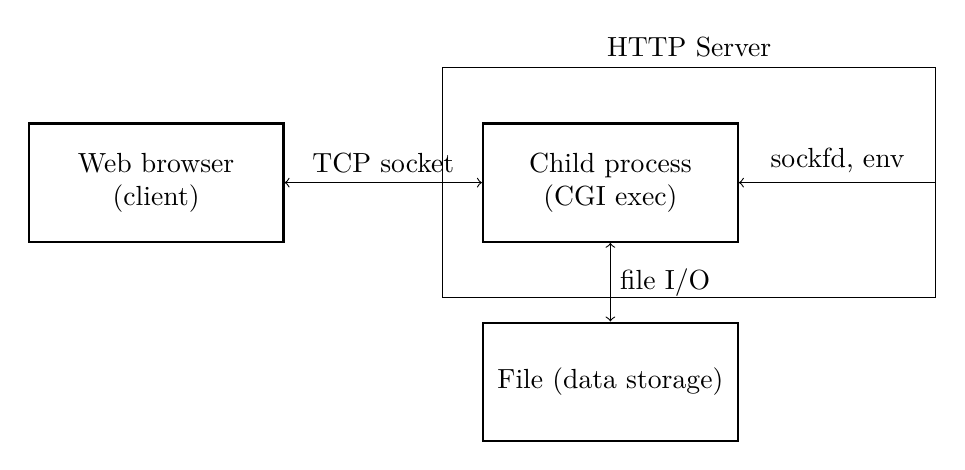
\begin{tikzpicture}
    \node[block] (a) {Child process (CGI exec)};
    \node[block,below=of a] (b) {File (data storage)};
    \node[draw,xshift=10mm,inner xsep=15mm,inner ysep=7mm,fit=(a),label={HTTP Server}](c){};
    \node[block,left=of c,xshift=-10mm] (d) {Web browser (client)};
    \draw[line, <->] (a) -- (b) node[midway,right] {file I/O};
    \draw[line, ->] (c.east) -- (a.east) node[midway,above] {sockfd, env};
    \draw[line, <->] (d) -- (a) node[midway,above] {TCP socket};
  \end{tikzpicture}
\end{frame}

\begin{frame}
  \frametitle{0x03 - Features}
  \framesubtitle{HTTP server}

  Features for the HTTP server

  \begin{itemize}
    \item<1-> We will not implement whole RFC 1945 (HTTP/1.0).
    \item<2-> Instead, implement \textit{subset} of the RFC 1945, barely able to serve the page
    \item<3-> Also, we will not implement whole RFC 3875 (CGI 1.1)
    \item<4-> Instead, implement \textit{subset} of the RFC 3875, barely able to run our CGI app
    \item<5-> Will be implemented without using any off-the-shelf libraries (planned)
  \end{itemize}
\end{frame}

\begin{frame}
  \frametitle{0x03 - Features}
  \framesubtitle{CGI guest book}

  Features for the CGI guest book app
  \begin{itemize}
    \item<1-> Take user input(nickname, message) through HTTP POST
    \item<2-> Store given data into the TSV-based simple data storage
    \item<3-> Implement CGI interface \& basic rendering engine
    \item<3-> libCGI will be used to parse CGI envvar / HTTP body (planned)
  \end{itemize}
\end{frame}

\end {document}
